% Här skriver jag all min brödtext kan man säga. Introduktion brukar jag ha som en egen fil om jag har en sådan.

%\begin{figure}[h]
%\centering
% Man kan inkludera en pdf som täcker nästan hela sidan.
%\includegraphics[width=\textwidth]{grafik/Inlamningsuppgift_5_min}
%\caption{Uppgiftsblad.}
%\label{fig:uppg}
%\end{figure}

%\clearpage

% * gör att rubriken inte numreras
\section*{Inledning}
Jag har fixat detta dokument där jag behållit och klistrat in olika exempel på hur man skriver ekvationer och tabeller med mera. Fritt fram att använda detta precis hur man vill. Hör gärna av er om ni har frågor. Är ingen latex-ninja men har spenderat otaliga timmar med att försöka få saker att se ut som jag vill. Google är najs. Dokumentet är inte perfekt men det kan i alla fall vara en början. Hoppas någon finner något av detta till nytta. 

Allt gott! // Martin

\subsection*{Tips om ekvationer}
Ett tips är att ha ett dokument där man klistrar in alla olika sorters ekvationer man skriver i latex. Då är det lätt att snabbt titta igenom och se om man hittar någon som liknar det man är ute efter för tillfället. Då är det oftast rätt enkelt att modifiera en gammal ekvation. Det kan nämligen vara lite pilligt att få till klamrar, matriser, kolumn-uppradning osv. när man håller på med lite mer komplicerade ekvationer.

\subsection*{Allmänt}
Som latex motor har jag valt att använda LuaLatex som är en vidareutveckling på latex. I stort sett allt som funkar till latex funkar också till LuaLatex så ni behöver inte googla lualatex ... om ni försöker hitta hur man löser något probem utan googla istället latex ... 

I början av varje källkodsfil försöker jag skriva en beskrivande kommentar så man får lättare att förstå vad den filen gör. 

\subsection*{Övrigt}
I setup\/hyphenations skriver man in ord som man vill radbryta/avstava på ett fördefinierat sätt. Man skriver in ord här som råkar bli fula i dokumentet helt enkelt. (Många av dessa ekvationer och bilden kommer från inlämningsuppgifterna i elektroniken. Jag har givetvis bytt ut lite siffror och ändrat så det går inte att återanvända...)

\newpage
\section{Hur man kommer igång}
\subsection{Hur man installerar mitt projekt}
Hämta projektet som ex en zip från min github på:

\url{https://github.com/martinclason/Martins-fina-latexmall}

Sedan är det bara att köra med vilken latex-miljö man vill! Så länge man använder LuaLatex som motor. Jag tycker dock att Overleaf är mycket smidigt att använda och rekommenderar det.

\url{https://www.overleaf.com}

\subsection{Om man vill köra Overleaf}
Skapa konto på overleaf. Välj upload project och ladda upp min zip som ni hämtade från github. I denna mapp göms det en del git-filer i .git mappen som den kommer säga att den inte kunde ladda upp men det är ingen fara.

För att kunna kompilera mitt projekt måste man välja LuaLatex som är en vidareutveckling av latex som renderingsmotor. Detta gör man genom att klicka på kugghjulet uppe i högra hörnet i overleaf och väljer LuaLatex som "Latex Engine". Nu bör allt fungera! i fortsättningen duplicerar ni detta projekt när ni vill skapa ett nytt dokument så hänger alla inställningar med.


% 

\clearpage
\section{Deluppgift a}

\subsection{Rita likströmsschema}
I denna deluppgift skall två komponentvärden bestämmas på sånt sätt att FET-transistorn... 

\begin{figure}[h]
\centering
% Man kan lägga in en koefficient ex. "width=0.5*\textwidth" för att få en bild som är halva textbredden.
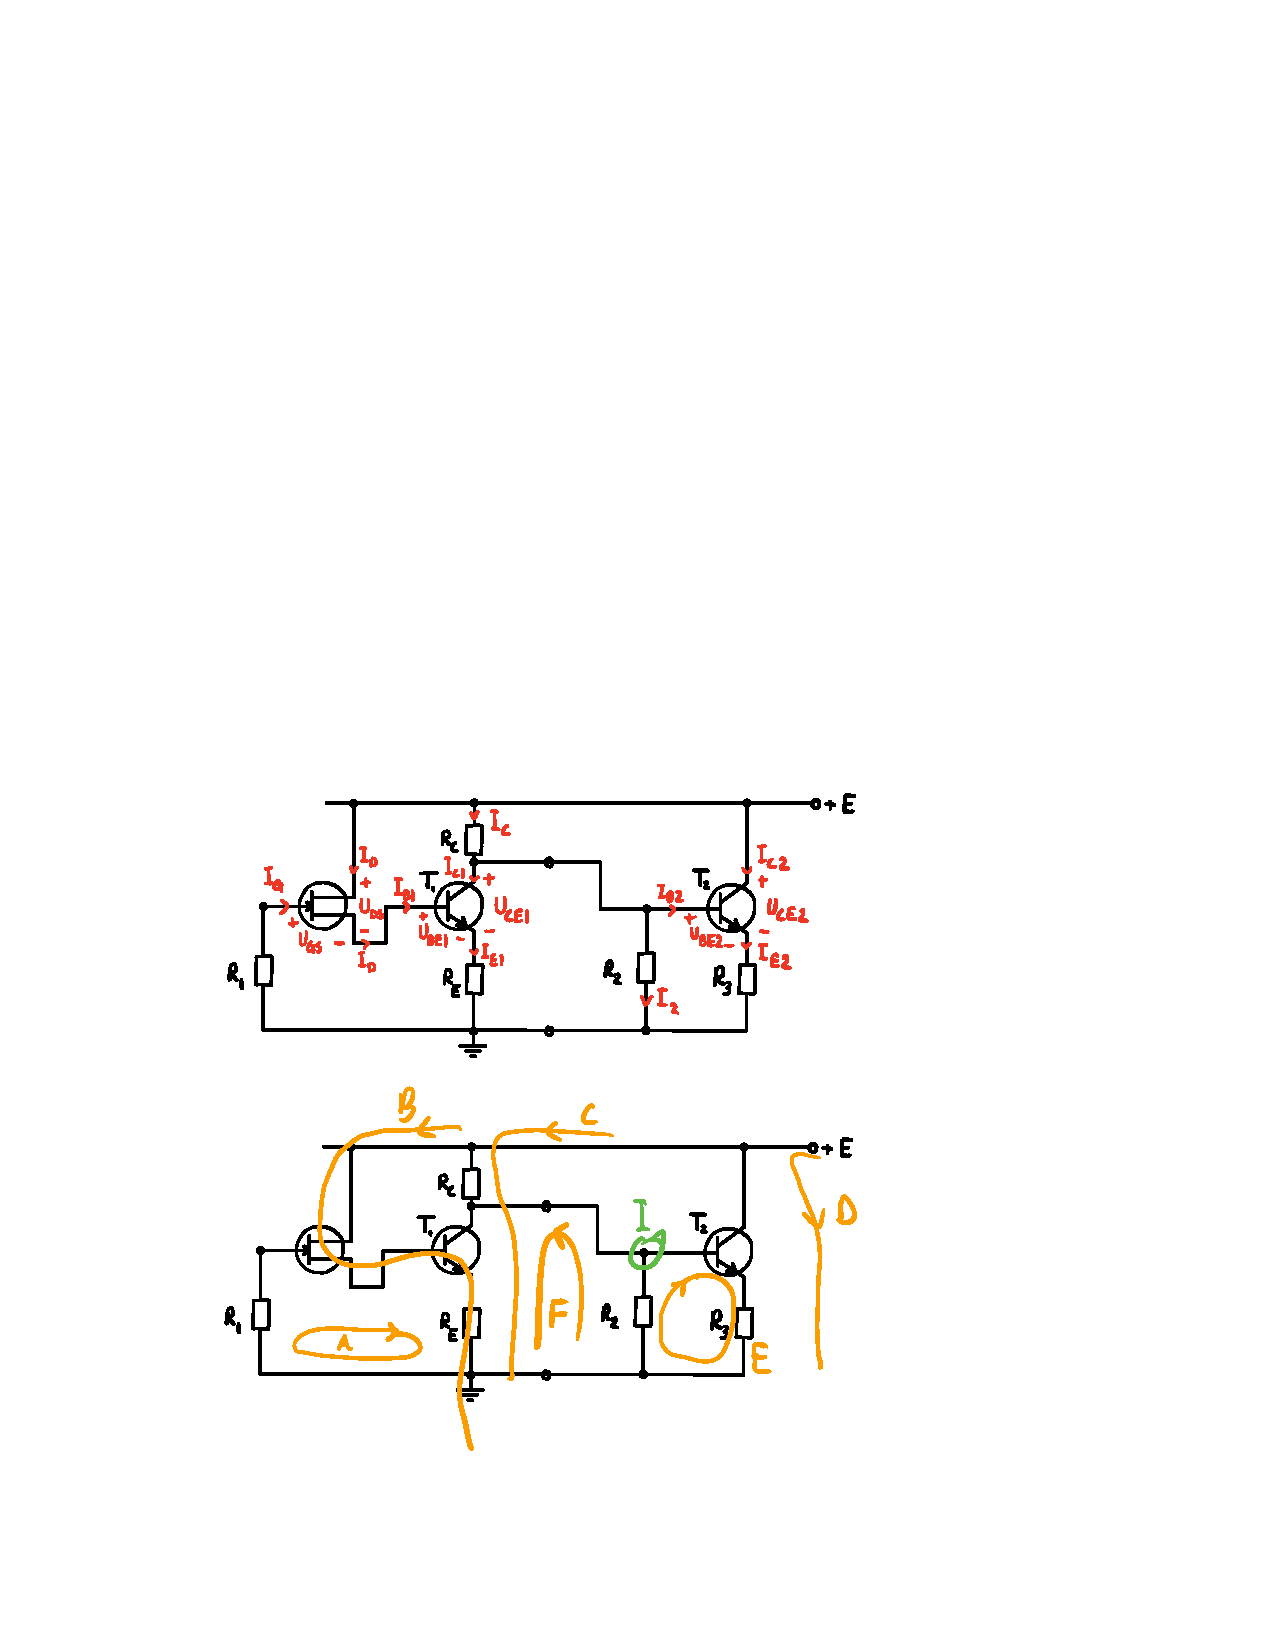
\includegraphics[width=\textwidth]{grafik/g1}
\caption{Likströmsschema och ekvationernas ursprung.}
\label{fig:g1}
\end{figure}

\begin{equation}
\begin{array}{l l}
\nonumber
\text{Givna värden:} & \text{Obekanta:}\\
\qquad R_1 = 1\text{ M\Omega} & \qquad R_E\\
\qquad R_2 = 10\text{ k\Omega} & \qquad I_{E1}\\
\qquad R_3 = 2\text{ k\Omega} & \qquad U_{GS}\\
\qquad R_L = 50\text{ \Omega} & \qquad R_{C}\\
\qquad E = 12\text{ V} & \qquad I_{C}\\
\qquad B = 50\text{  } & \qquad U_{CE1}\\
\qquad I_{DSS} = 12\text{ mA} & \qquad I_{E2}\\
\qquad U_{p} = -4\text{ V} & \qquad I_{B2}\\
\qquad U_{BE1} = 0.7\text{ V} & \qquad I_{2}\\
\qquad U_{BE2} = 0.7\text{ V} & \qquad I_{C1}\\
\qquad I_{G} = 0\text{ A} & \qquad I_{B1}\\
\qquad U_{DSQ} = 10\text{ V} & \qquad I_{C2}\\
\qquad U_{CEQ2} = 2\text{ V} & \qquad I_{D}
\end{array}
\end{equation}

\begin{equation}
  \left.
\begin{IEEEeqnarraybox}[\IEEEeqnarraystrutmode \IEEEeqnarraystrutsizeadd{2pt}{2pt}][c]{rCl} 
\varphi_e &=& 0 \\
e(t) &=& 10\sin{1000t+\varphi_e}
  \end{IEEEeqnarraybox}
  \, \right\} \Rightarrow \left\{ \,
  \begin{IEEEeqnarraybox}[
    \IEEEeqnarraystrutmode
    \IEEEeqnarraystrutsizeadd{7pt}
    {7pt}][c]{rCl}
    E &=& 10 \text{ V}
    \\
    \omega &=& 1000 \text{ rad/s}
  \end{IEEEeqnarraybox}
  \right.
  \label{eq:E}
\end{equation}


Vissa av dessa symboler har kända värden och således har vi 13 st obekanta. Att lösa ut dessa kräver 13 ekvationer. Vi applicerar likströmsanalys... Eftersom vi söker en viss arbetspunkt så blir $U_{DSQ}$ och $U_{CEQ2}$ istället $U_{DS}$ respektive $U_{CE2}$.


% rrcl betyder att det ska vara 4 olika kolumner. Varje bokstav avgör vilken justering den kolumnen ska ha. r betyder högerjust., l=vänster, c=center... 
% Man avgränsar kolumnerna med hjälp av &. I det här fallet vill vi ha alla = ovanför varandra så vi skriver &=& på varje rad.
\begin{IEEEeqnarray}{rrCl}
\textnormal{A:} \quad & U_{BE1} + R_EI_{E1} + R_1I_G + U_{GS} &=& 0 \\
\textnormal{B:} \quad & -E + U_{DS} + U_{BE1} + R_EI_{E1} &=& 0 \\
\textnormal{C:} \quad & -E + R_CI_C + U_{CE1} + R_EI_{E1} &=& 0
\end{IEEEeqnarray}

Vi har även följande samband från bla. teori om transistorernas egenskaper.

\begin{IEEEeqnarray}{rCl}
I_{E1} &=& I_{C1} + I_{B1} \\
I_{D} &=& I_{B1} \\
I_{D} &=& I_{DSS}\left( 1 - \frac{U_{GS}}{U_p}\right)^2, U_p < U_{GS} <  0
\end{IEEEeqnarray}

Vi har nu skrapat ihop till några ekvationer...

% \left betyder att det finns en \right senare som hänger ihop med denna. Ex. att två parentesers storlek ska matcha varandra. 
% Om man inte vill ha något till höger skriver man \right. så renderas inget på högersidan.
\begin{IEEEeqnarray}{c}
\left\{ \begin{IEEEeqnarraybox}[
    \IEEEeqnarraystrutmode
    \IEEEeqnarraystrutsizeadd{7pt}
    {7pt}][c]{rcl}
    \nonumber
    U_{BE1} + R_EI_{E1} + R_1I_G + U_{GS} &=& 0 \\
    U_{BE2} + R_3I_{E2} - R_2I_{2} &=& 0 \\
    I_{B2} + I_{2} - I_{C} + BI_{B1} &=& 0 \\
    I_{E1} &=& I_{B1}\left( B + 1\right) \\
    I_{E2} &=& I_{B2}\left( B + 1\right)\\
    I_{B1} &=& I_{DSS}\left( 1 - \frac{U_{GS}}{U_p}\right)^2
  \end{IEEEeqnarraybox}
  \right.
\end{IEEEeqnarray}

Detta system matas in i Matlab och vi får då ut följande numeriska värden på de obekanta.

\begin{IEEEeqnarray}{c}
\left\{ \begin{IEEEeqnarraybox}[
    \IEEEeqnarraystrutmode
    \IEEEeqnarraystrutsizeadd{7pt}
    {7pt}][c]{lcll}
    \nonumber
    U_{GS} && &= -2 \text{ V} \\
    I_{C} &=& 15407/100000 \text{ A } &= 154.07 \text{ mA} \\
    I_{B2} &=& 1/10200 \text{ A} &\approx 98.0392e-05 \text{ \mu A} \\
    R_{C} &=& 130000/15407 \text{ \Omega} &\approx 8.43772 \text{ \Omega} \\
    R_{E} &=& 1300/153 \text{ \Omega } &\approx 8.49673 \text{ \Omega}
  \end{IEEEeqnarraybox}
  \right.
\end{IEEEeqnarray}

Således har vi bestämt värden på...

\newpage

\section{Deluppgift b}
Nu skall utspänningen $u_{ut}(t)$ bestämmas som funktion av inspänningen $u_{in}(t)$ då $u_{in}(t)=\sin (10^3t) [mV]$. Vi vet att

% Det här är lite enklare sätt att skriva ekvationer men är inte lika kraftfullt som IEEEeqnarray ex.
\begin{equation}
u_{ut}(t)=F\cdot u_{in}(t)
\label{eq:ub}
\end{equation}

där $F$ är förstärkningsfaktorn. Vi räknar därför ut förstärkningsfaktorn.

\subsection{Fler ekvationer}

\begin{IEEEeqnarray}{rCl}
R_4 &=& R_C \parallelsum R_2 = \frac{R_CR_2}{R_C + R_2} \\
R_7 &=& R_8 \parallelsum R_L = \frac{R_8R_L}{R_3 + R_F}
\end{IEEEeqnarray}

\begin{IEEEeqnarray}{C} 
\nonumber
u_{ut}(t) \approx \frac{R_5\left(1 + h_{21}\right)}{\frac{1}{g_m} + h_{11} + R_{E}\left(1 + h_{21}\right)} u_{in}(1000t) \quad \text{ [mV]} \\
\Leftrightarrow \nonumber \\
\nonumber
u_{ut}(t) \approx \frac{R_5\left(1 + h_{21}\right)}{\frac{1}{g_m} + h_{11} + R_{E}\left(1 + h_{21}\right)} \sin(1000t) \quad \text{ [mV]} \\
\Leftrightarrow \nonumber \\
u_{ut}(t) \approx \frac{R_5\left(1 + h_{21}\right)}{\frac{1}{g_m} + h_{11} + R_{E}\left(1 + h_{21}\right)} \sin(1000t) \quad \text{ [mV]} \\
\Leftrightarrow \nonumber \\
u_{ut}(t) \approx 0.927132 \cdot \sin(1000t) \quad \text{ [mV]}
\label{eq:f1}
\end{IEEEeqnarray}

\newpage

\section{Lite exempel på hur man får till olika ekvationer etc}

\subsection{Invärden}
\begin{table}[h!]
\centering
\begin{tabular}{|l| }
  \hline
  Komponentvärden \\
 \hline
 $R_1=500\text{ \Omega}$\\
 $R_2=4\text{ \Omega}$\\
 $C_1=2\text{ \mu F}$\\
 $C_2=0.5\text{ \mu F}$\\
 $L_1=1.5\text{ H}$\\
 $L_2=8\text{ mH}$\\
 ${N_1}/{N_2}=10$\\
 \hline
\end{tabular}
\caption{Komponentvärden i uppgiften.}
\label{table:komponentvärden}
\end{table}

\small
\begin{equation}
\begin{pmatrix}
\dfrac{1}{R_2}+\dfrac{1}{R_4}+\dfrac{1}{R_6} & -\dfrac{1}{R_4} & -\dfrac{1}{R_6} \\[2ex]
-\dfrac{1}{R_4} & \dfrac{1}{R_3}+\dfrac{1}{R_4}+\dfrac{1}{R_7} & 0 \\[2ex]
0 & 0 & -\dfrac{1}{R_{10}}
\end{pmatrix}
\begin{pmatrix}
V_1 \\[3ex]
V_2 \\[3ex]
V_4
\end{pmatrix}
=
\begin{pmatrix}
-\dfrac{E_4}{R_2} \\[2ex]
\dfrac{E_1}{R_9}-I_{02} \\[2ex]
-I_{01}
\end{pmatrix}
\end{equation}

\normalsize


\begin{equation}
\begin{array}{l l l}
R_1 = 1\text{ k\Omega} & E_1=3\text{ V} & I_{01}=1\text{ mA}\\
R_2 = 6\text{ k\Omega} & E_2=6\text{ V} & I_{02}=2\text{ mA}\\
R_3 = 6\text{ k\Omega} & E_3=2\text{ V} & \\
R_4 = 2\text{ k\Omega} & E_4=E_2+E_3=8\text{ V} & \\
R_5 = 8\text{ k\Omega} & & \\
R_6 = 5\text{ k\Omega} & & \\
R_7 = 10\text{ k\Omega} & & \\
R_8 = 10\text{ k\Omega} & & \\
R_9 = 12\text{ k\Omega} & & \\
R_{10} = 1\text{ k\Omega} & &
\end{array}
\end{equation}

\begin{equation}
\begin{array}{l l}
U_0=-1.234567...\text{ V}\approx -1.23\text{ V} & \text{eller} \\
U_1=1.234567...\text{ V}\approx \boxed{1.23\text{ V}} \qquad & \text{med referensriktning motsatt den för $U_0$} \\
R_0=1.234567...\text{ \Omega}\approx \boxed{1.23 \text{ k\Omega}} &
\end{array}
\label{eq:svar}
\end{equation}


